Consideremos un sistema de ecuaciones diferenciales ordinarias (EDO) descrito por 
\begin{equation}
\dot{\mathbf{x}}(t) = f(\mathbf{x}(t),t)
\label{eq:ode}
\end{equation}
con $t$ el parametro que describe la evolución del sistema y $\flowci$ la trayectoria o \textbf{flujo} de la solución que en $t_0$ se encuentra en $\xo$. En la mayoría de los sistemas físicos, el parámetro $t$ describe al tiempo, i.e., $t \in \mathbb{R}^+$, y al sistema de ODE se le conoce como sistema dinámico.

Pocos son los casos en donde la solución a $\dot{\mathbf{x}}(t)$ se puede obtener de manera analítica y, por tanto, estudiar las familias de soluciones para diferentes condiciones iniciales termina siendo, casi siempre, un estudio indirecto o aproximado. Se han considerado varias formas para darle la vuelta a este problema y, en los esfuerzos de lo aproximado, una de las soluciones más prácticas ha sido discretizar al parámetro temporal $t$ de (\ref{eq:ode}) y encontrar, en saltos discretos de $t$, el ``estado actual'' del sistema dado un ``estado anterior''.

Gracias a que hoy en día existe poder de cómputo para hacer muchas operaciones simples en relativamente poco tiempo, se ha explotado el estudio y uso de métodos iterativos para obtener $\flowci$, siendo de gran utilidad en los últimos años. Éstos se conocen como \textbf{métodos numéricos de integración de ecuaciones diferenciales}. Con estos métodos se puede, en la mayoría de los casos, definir una condición inicial $\xo := \mathbf{x}(t_0)$ y obtener la solución para esta condición particular. Sin embargo, no siempre es suficiente obtener la solución de una única condición inicial dada y, muchas veces, interesa todo una familia de soluciones alrededor de un punto $\xo$ de interés. Esto puede pasar, por ejemplo, en aceleradores de partículas que disparan paquetes de onda como si fuesen ``gotas" sujetas a algún campo externo. En mecánica de fluidos es interesante estudiar parcelas de fluidos y, con la representación lagrangiana de las ecuaciones de Navier-Stokes, ver cómo evolucionan estas parcelas en el tiempo; ésta es una rama muy utilizada por los métodos computacionales, ya que por las no linealidades de las ecuaciones de Navier-Stokes, ha sido muy difícil obtener soluciones analíticas sin hacer un montón de aproximaciones previas. En sistemas de muchos cuerpos también se ha pensado en familias de soluciones cercanas, ya que difícilmente se conocen las condiciones iniciales de todo el sistema con una precisión profunda, de hecho, en todos los sistemas donde las condiciones iniciales pueden no saberse con exactitud, un método exhaustivo sería el conseguir todas las soluciones de las posibles condiciones iniciales para estos sistemas. Una rama muy relacionada a lo anterior son los métodos de Montecarlo, donde, en el caso de las EDO, se consigue una distribución inicial de condiciones iniciales y se obtiene cada una de las soluciones para éstas. 
En un plano más general, el mundo de las ecuaciones diferenciales ordinarias ha estudiado exhaustivamente los campos vectoriales que generan las ecuaciones de la forma (\ref{eq:ode}). Ha habido gran interés en entender el comportamiento de órbitas periódicas y puntos singulares o, más generalmente, la topología del campo vectorial que representa las soluciones de las ecuaciones. Se han desarrollado métodos para encontrar estructuras hiperbólicas en el espacio fase y métricas para catalogar el comportamiento de las soluciones. Algunos de los resultados teóricos para esto son el número de Euler, que categoriza la topología del espacio, las secciones de Poincaré, que son representaciones de la solución en un espacio de menor dimensionalidad, donde normalmente se busca que no sea tangente a las soluciones para entender cómo éstas cruzan dichas secciones que describe, los exponentes de Lyapunov, que estudia la separación de soluciones cercanas a una condición inicial dada, la derivada de Lie, que compara al campo vectorial de (\ref{eq:ode}) contra otro campo vectorial, la linealización de Grobman-Hartman, que toma la parte lineal de $\dot{\mathbf{x}}(t)$ en localidades suficientemente pequeñas y analiza qué quiere decir ``suficientemente'', entre otras. 
%%REFERENCIAS NECESARIAS EN EL PÄRRAFO ANTERIOR.

Muchas de estas preguntas podrían responderse si, en vez de encontrar $\flowci$ para una condición $\mathbf{x}_0$ dada, se tuviera una vecindad inicial $\U$ alrededor de $\mathbf{x}_0$ (que llamaremos $\Uxo$) y se encuentra el flujo para toda esta parcela. Parecería una idea idéntica a las simulaciones de Montecarlo, pero la gran diferencia es que en Montecarlo se integra cada solución de manera independiente y aquí se integra toda la vecindad $\Uxo$ a la vez. Ésta es la principal motivación detrás del Transporte de Jets (TJ); dada la vecindad inicial $\U_{\xo}$ alrededor de $\xo$ parametrizada por el vector $\mathbf{\xi}$, se busca obtener $\flowxi$ y evaluar $\xi$ en $\Uxo$ para obtener $\flowU$, la deformación de la vecindad $\U_{\xo}$ al tiempo $t$. La idea operativa computacional del TJ es muy similar a la de cualquier método numérico de integación de EDO: discretiza los pasos del parámetro de evolución (tiempo) en intervalos $h_n$ y encuentra un método iterativo para conseguir el siguiente punto del flujo $\flowci$. En la figura \ref{fig:FIGURA!} se observa un esquema cualitativo de la idea del transporte de jets.

%FIGURA!

Merece la pena ilustrar dicha discretización con un método muy sencillo e intuitivo aunque, al  no ser tan preciso, se usará otro para el desarrollo de esta tesis.

Sabemos, por definición, que 
\begin{equation*}
 \dot{\mathbf{x}}(t) = \lim_{h\to 0} \frac{\mathbf{x}(t+h)-\mathbf{x}(t)}{h}.
\end{equation*}  

Si tomamos $h$ \textit{suficientemente pequeña}, aunque finita, podemos aproximar
\begin{equation*}
 \mathbf{x}(t+h) \approx \mathbf{x}(t) + h \dot{\mathbf{x}}(t)
\end{equation*}

que, si tomamos en cuenta que $\dot{\mathbf{x}}(t) = f(\mathbf{x}(t),t)$ y que $h$ es un paso de integración, se obtiene
 
\begin{equation}
 \mathbf{x}_{n+1} = \mathbf{x}_n + h f(\mathbf{x}_n,t_n)
 \label{eq:euler} 
\end{equation}

que se conoce como el \textbf{Método de Euler}. Así, dada $\xo$ se puede obtener $\flowci$ iterando (\ref{eq:euler}) hasta llegar a $t$ en pasos de $h$.

Ahora, para la evolución del TJ se parametriza a la vecindad $\U_{xo}$ usando un polinomio $P_{t_0,\xo}(\xi)$ alrededor de $\xo \in \mathbb{R}^n$ 
\begin{equation*}
 P_{t_0,\xo}(\xi) = P_{0,\xo}(\xi) = \xo + \xi = \xo + \left( \xi_1, \xi_2, ..., \xi_n \right)^T
\end{equation*} 

y se evalúa con el método de Euler (o cualquier otro) para obtener el flujo de $\Uxo$ en algún tiempo $t$ posterior $\flowU$
\begin{equation*}
P_{1,\xo}(\xi) := P_{t_0+h,\xo}(\xi) = P_{t_0,\xo}(\xi) + h f(P_{0,\xo},t_0) = \xo + \xi + h f(\xo + \xi).
\end{equation*}

Así, se puede extender el método de Euler al TJ 
\begin{equation}
 P_{t_n,\xo}(\xi) = P_{n,\xo}(\xi) = P_{n-1,\xo}(\xi) + h f(P_{n-1,\xo}(\xi),t_{n-1})
 \label{eq:eulerU}
\end{equation}

donde $P_{n,\xo}(\xi)$ representa al flujo $\flowxi$. Basta evaluar éste polinomio en $\Uxo$ para obtener $\flowU$\footnote{$\flowxi$ no necesariamente debe ser evaluado en toda una vecindad $\Uxo$; puede, también, ser en un único punto $\xi =\delta \mathbf{x}$ y obtener el flujo para $\phi(t;t_0,\xo + \delta \mathbf{x})$}.

Es importante notar que la solución $\flowci$ o el conjunto de soluciones $\flowU$ son sensibles al método de integración utilizado para encontrarlas dado que la solución construida es una aproximación. Se recomienda al lector, si le interesa, leer el desarrollo explícito en \cite{p-palau} para ver estas diferencias.

Para ilustrar un poco lo anterior, merece la pena desarrollar un ejemplo que motive el uso del Transporte de Jet.

Sea
\begin{align}
\dotx = f(\mathbf{x},t) = \left[ \begin{array}{cc}
 0 & -1  \\
 1 & 0  \\
\end{array} \right] \left( x_1, x_2 \right)^T
\label{eq:center}
\end{align}
un campo vectorial que describe centros alrededor de $x_0 = (0,0)$. 

Si se toma $P_{0,\xo} = (x_{1_0},x_{2_0}) + (\xi_1,\xi_2)$ como la vecindad inicial, podemos desarrollar ``a mano'' el transporte de Jet, donde, usando el método de Euler tenemos

\begin{align*}
\mathbf{x}_1 &= P_{1,\xo}(\xi) = P_{0,\xo}(\xi) + h f(P_{0,\xo}(\xi),t_0) \\
&= (x_{1_0} - h x_{2_0}, h x_{1_0} + x_{2_0} )^T + \left[ \begin{array}{cc}
 1 & -h  \\
h & 1  \\
\end{array} \right] (\xi_1,\xi_2)^T.
\end{align*} 

El primer término de $\mathbf{x}_1$ corresponde al primer paso de integración de $\xo$ sin el transporte de jets. El segundo término es la solución de las ecuaciones variacionales de primer order para el primer paso con el método de Euler, o dicho de otra manera, una aproximación lineal de soluciones cercanas a $\xo$ parametrizadas por las $\xi$'s. Gracias a esta parametrización, es natural pensar en obtener soluciones cercanas simplemente evaluando $\xi$ en $P_{1,\xo}(\xi)$ o, más generalmente, en $P_{n,\xo}(\xi)$. De este modo, el TJ se plantea a ser un buen método para hacer simulaciones de Montecarlo de manera muy rápida, ya que habría que hacer una sola integración de $\U_{\xo}$ y después simplemente evaluar los polinomios. La única desventaja en esto es que la integración de $\U_{\xo}$, al operar siempre con polinomios y no con números, suele ser más lenta que la de una única trayectoria que pasa por $\xo$ en $t_0$. Naturalmente, el tiempo en donde uno u otro método es mejor es discutible y dependerá fuertemente de la complejidad y la dimensionalidad de las ecuaciones presentes en el sistema\footnote{Para una discusión más a fondo sobre este tema, revisar la sección \ref{sec:}, donde se hacen varios benchmarks en relación al tiempo de cómputo y la memoria utilizada.}.

Se podría seguir haciendo el desarrollo del TJ iterativamente con el método de Euler. Por ejemplo, el segundo paso quedaría como 
\begin{align*}
\mathbf{x}_2 =& P_{2,\xo}(\xi) = P_{1,\xo}(\xi) + h f(P_{1,\xo}(\xi),t_n) \\
=& (x_{1_0} - h x_{2_0}, h x_{1_0} + x_{2_0} )^T + \left[ \begin{array}{cc}
 1 & -h  \\
h & 1  \\
\end{array} \right] (\xi_1,\xi_2)^T \\ 
&+ h \left( \left[ \begin{array}{cc}
 0 & -1  \\
 1 &  0  \\
\end{array} \right] \left( (x_{1_0} - h x_{2_0}, h x_{1_0} + x_{2_0} )^T + \left[ \begin{array}{cc}
 1 & -h  \\
h & 1  \\
\end{array} \right] (\xi_1,\xi_2)^T \right) \right) \\
=& \left[ \begin{array}{c}
x_{1_0} - h^2x_{1_0} - 2h x_{2_0}  \\
2h x_{1_0} + x_{2_0}  - h^2x_{2_0}  \\
\end{array} \right] + \left[ \begin{array}{cc}
 1-h^2 & -2h  \\
2h & 1-h^2  \\
\end{array} \right] (\xi_1,\xi_2)^T
\end{align*}
 
y así sucesivamente. Una vez que se obtiene $P_{n,\xo}(\xi)$ basta con evaluarlo para valores $\mathbb{\xi}$ \textit{suficientemente pequeños} para encontrar las soluciones en la vecindad de $\xo$. En la figura \ref{fig:center-evals} se evalúa $\flowxi$ para distintos valores de $t$ en vecindades $\Uxo$ dadas por círculos de distinto radio.

se pueden ver las evaluaciones de $P_{n,\xo}(\xi)$ para distintos valores de $t_n$ y de $\xi$ alrededor del punto singular $\xo = (0,0)$.

%FIGURA!
\begin{figure}[h!]
 \centering
 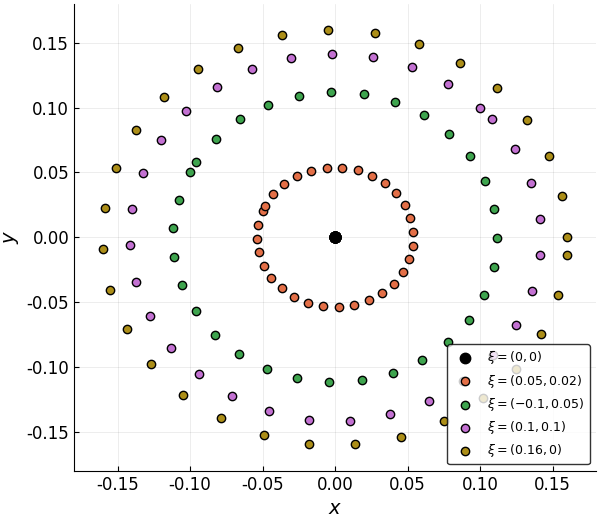
\includegraphics[width=0.8\linewidth]{euler-jt-evaluations-center}
 \caption{Transporte de jets para la ecuación (\ref{eq:center}) con condición inicial $\xo = (0,0)^T$ usando el método de Euler para $\Uxo$ parametrizada en un círculo $\xi(\tau) = r\left( \cos(\tau),\sin(\tau) \right)$ para un intervalo temporal $[0,2\pi]$ en pasos de $h=10^{-4}$. Se evaluó la solución para los distintos $r$'s marcados en la gráfica, en intervalos de $1000h$.}
 \label{fig:center-evals}
\end{figure}

Notemos que (\ref{eq:center}) corresponde a un sistema hamiltoniano cuyas soluciones en el espacio fase viven en las curvas de nivel dadas por
\begin{equation*}
H(\mathbf{x}) = \frac{1}{2} \left( x_1^2 + x_2^2 \right),
\end{equation*} 
con solución analítica
\begin{align}
 x_1(t) &= x_{01}\cos{(t)} - x_{02}\sin{(t)} \nonumber \\
 x_2(t) &= x_{01}\sin{(t)} + x_{02}\cos{(t)}.
 \label{eq:center_analytical}
\end{align}

En la figura \ref{fig:center_anal_comparison} se muestran distintas comparaciones de la integración numérica contra las soluciones analíticas de (\ref{eq:center_analytical}).

%FIGURA! 
\begin{figure}[h!]
\centering
\begin{subfigure}{0.49\textwidth}
	\centering
	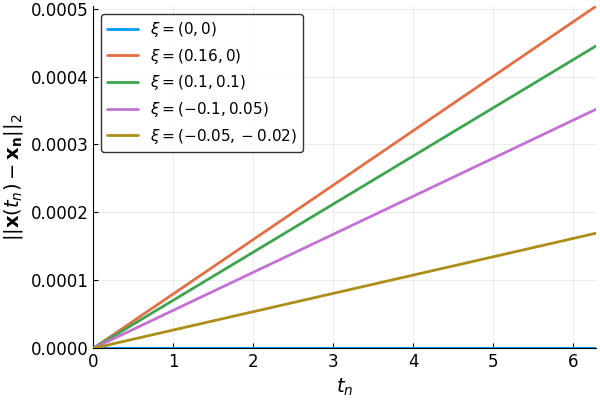
\includegraphics[width = \textwidth]{euler-vs-analytical_center}
	\caption{Norma de la diferencia entre la solución real y evaluaciones de la solución numérica para distintos valores de $\xi$ marcados en la gráfica. Se puede observar un crecimiento lineal del error numérico, lo cual es una de las consecuencias de usar el método de Euler.}
	\label{fig:center-eu_vs_anal}
\end{subfigure}
%
\begin{subfigure}{0.49\textwidth}
	\centering
	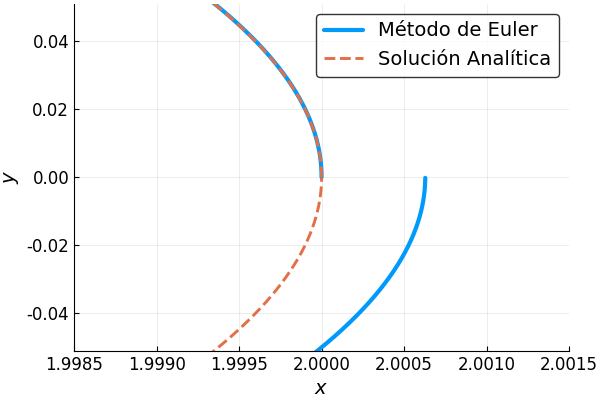
\includegraphics[width = \textwidth]{euler-method_error}
	\caption{Sección del espacio fase donde se observan la solución analítica y la solución numérica para pasos de $h=10^{-4}$ con cóndición inicial $\xo = (2,0)$. \\ \\}
	\label{fig:center_not-closed}
\end{subfigure}
\caption{Diferencias numéricas entre el método de Euler y la solución analítica para \ref{eq:center}}
\label{fig:center_anal_comparison}
\end{figure}


Queda claro que el desarrollo de TJ necesita de un álgebra polinomial para poder evaluar los distintos $P_{j,\xo}(\xi)$ que definen al campo vectorial en cada uno de sus pasos. El problema de evolucionar una vecindad $\U_{\xo}$ dado un sistema dinámico $\dot{\mathbf{x}}(t) = f(t,\mathbf{x}(t))$ se reduce al problema de saber cómo se evalúan distintos polinomios en cada paso de integración, así como la definición computacional de sus operaciones. Hay muchos detalles a considerar en este problema: ¿Qué paso de integración se deberá usar para conseguir la evolución temporal de las soluciones? ¿Cómo medimos el error respecto a la solución real? ¿Existe alguna forma de controlar el error que arrojan el método de integración y la propagación de jets del TJ? ¿Cuál es la complejidad de las operaciones para la aritmética de polinomios? En la siguiente sección \ref{sec:alg_poli} se desarrolla el álgebra polinomial y sus operaciones tal como son implementadas en el TJ y se ahonda en esta discusión. En la sección \ref{sec:taylor-metodo} se hace el desarrollo del método de Taylor como integrador computacional adaptativo de sistemas de EDO. En el siguiente capítulo se desarrollarán herramientas a partir del transporte de jets y sus características así como sencillos ejemplos ilustrativos para cada una de ellas.


\section{Álgebra Polinomial}
\label{sec:alg_poli}

La necesidad del álgebra polinomial se vuelve imperativa para el TJ como hemos visto en la sección anterior. Haremos la construcción de manera formal donde denotaremos  dicha álgebra como $\algpol$ donde $\pk$ es el conjunto de \textbf{polinomios de orden $n$ con coeficientes en el campo $\mathbb{K}$} tal que, si  $P(x) \in \pk$, éste se define como
$$P = P(x) := \polk{p_k} $$
con $P: \mathbb{C} \to \mathbb{K}$ una función analítica y $p_k \in \mathbb{K} \  \forall i \in [0,n]$.

Esta sección se divide en tres: la primera sobre construcción formal del álgebra en una variable vía la demostración de sus propiedades de campo, la segunda sobre el desarrollo de las operaciones para las funciones estándar dentro de ésta álgebra. La tercera sección es la extensión de dicha álgebra a más variables, para poder trabajar a cualquier dimensionalidad

%		- It may be necessary to analize how different independet variables imply that A(x) != A(b).

\subsection{Construcción del Álgebra}
\label{sec:alg_field}

Inspirado en la aritmética usual en $\mathbb{C}$ o $\mathbb{R}$, podemos definir $(+,\cdot)$ para $\algpol$ de la siguiente manera:

Sean $A,B \in \pk$ con $A = \polk{a_k}$ y $B = \polk{b_k} \ a_k,b_k \in \mathbb{K} \ \forall k \in [0,n]$, entonces, para la suma, notemos que
\begin{align*}
\polk{a_k} + \polk{b_k} =& a_0 + a_1 x + \cdots a_n x^n + b_0 + b_1 x + \cdots + b_n x^n \\
=& (a_0 + b_0) + (a_1 + b_1) x + \cdots + (a_n + b_n)x^n = \polk{(a_n + b_n)} 
\end{align*}
así, se define \textbf{$+$}  en $\pk$ como
\begin{equation}
A + B = \polk{(a_k + b_k)}.
\label{eq: polsum}
\end{equation}

Para el producto, notemos que
\begin{align*}
\polk{a_k}\cdot\polk{b_k} =& (a_0 + a_1 x + \cdots + a_n x^n)\cdot(b_0 + b_1 x + \cdots + b_n x^n) \\
=& (a_0b_0) + (a_1b_0 + a_0b_1) x + (a_2b_0 + a_1b_1 + a_0b_2) x^2 + \cdots + \\
+& \sum_{j=0}^n a_{n-j}b_j x^n + \mathcal{O}(x^{n+1}) = \polk{ \polj{a_{k-j}b_j } }
\end{align*}

así, se define \textbf{$\cdot$}  en $\pk$ como

\begin{equation}
A \cdot B = \polk{\sum_{j=0}^k a_{k-j}b_j}.
\label{eq: polprod}
\end{equation}
Aún cuando las operaciones están definidas inspiradas en la aritmética de los números, $\mathbb{K}$ puede ser cualquier campo arbitrario.

\begin{proposicion}
Para $\mathbb{K} = \mathbb{R}$ o $\mathbb{C}$, $\algpol$ forma un campo.
\label{prop:alg-field}
\end{proposicion}

\begin{proof}
Basta probar las nueve propiedades de campo con las operaciones de \ref{eq: polsum} y \ref{eq: polprod}.
Sean $A$, $B$ y $C \in \pk$
\begin{enumerate}

 \item $ A + B = B + A $
 \begin{proof}
  \begin{align*}
   A + B =& \polk{a_k} + \polk{b_k}  = \polk{(a_k + b_k)} \\ 
   =& \polk{(b_k + a_k)} = \polk{b_k} +     \polk{a_k} = B + A
  \end{align*}
 \end{proof}
 
 \item A + (B+C) = (A+B) + C
 \begin{proof}
  \begin{align*}
   A + (B+C) =& \polk{a} + \polk{(b_k+c_k)} = \polk{(a_k + (b_k + c_k))} \\
   =&  \polk{((a_k + b_k) + c_k)} = \polk{(a_k+b_k)} + \polk{c_k} \\
   =& (A+B) + C 
  \end{align*}
 \end{proof}
 
 \item $\exists \  \bm{0} \in \pk \text{ tal que }  \bm{0} + A = A $
 \begin{proof}
 Sea $\mathbb{0} = \bm{0}(x) = \polk{\sigma_k}$ donde $\sigma_k = 0 \ \forall k \in [0,n]$, así 
  \begin{align*}
  \bm{0} + A = \polk{(\sigma_k + a_k)} = \polk{(0 + a_k)} = \polk{a_k} = A
  \end{align*}
 \end{proof}
 
 \item $\exists \ {-A} \in\pk  \text{ tal que } A + (-A) = 0 $
 \begin{proof}
 Sea $-A = -A(x) = \polk{\mathrm{a}_k}$ donde $\mathrm{a}_k = -a_k \ \forall k \in [0,n]$, así
  \begin{align*}
   A + (-A) = \polk{(a_k + \mathrm{a}_k)} = \polk{(a_k + (-a_k))} = \polk{0} = \bm{0}
  \end{align*}
 \end{proof}
 
 \item $ A\cdot B = B\cdot A $
 \begin{proof}
 Hay que probar, básicamente, que $\sum_{j=0}^k{a_{k-j}b_j} = \sum_{j=0}^k{b_{k-j}a_j}$:
  \begin{align*} 
   \sum_{j=0}^k{a_{k-j}b_j} =& \sum_{i=0}^k{a_ib_{k-i}} \text{ con } i = k - j \\
   =& \sum_{i=0}^k{ b_{k-i}a_i } = \sum_{j=0}^k { b_{k-j}a_j }
  \end{align*}
  $\therefore A\cdot B = B\cdot A$.
 \end{proof}
 
 \item $ (A \cdot B) \cdot C = A \cdot (B \cdot C) $
 \begin{proof}
 Por un lado
  \begin{align*}
  A \cdot (B \cdot C) =& \polk{a_k}\ \polk{ \polj{b_{k-j}c_j} } = \polk{\big(  \sum_{j=0}^ka_{k-j}\sum_{i=0}^jb_{j-i}c_i \big)} \\
  =& \polk{\big(  \sum_{r+j=k}a_r\sum_{p+i=j}b_pc_i \big)} = \polk{\big(  \sum_{r+j=k}\sum_{p+i=j}a_rb_pc_i \big)} \\
  =& \polk{\big(  \sum_{r+p+i=k}a_rb_pc_i \big)} 
  \end{align*}
  por otro
    \begin{align*}
  (A \cdot B) \cdot C =& \polk{ \polj{a_{k-j}b_j} }\ \polk{c_k} = \polk{\big( \sum_{i=0}^ja_{j-i}b_i  \sum_{j=0}^kc_{k-j} \big)} \\
  =& \polk{\big(  \sum_{r+j=k}(\sum_{p+i=r}a_pb_i) c_j \big)} = \polk{\big(  \sum_{r+j=k}\sum_{p+i=r}a_pb_ic_j \big)} \\
  =& \polk{\big(  \sum_{p+i+j=k}a_pb_ic_j \big)} 
  \end{align*}
  
  Basta ver que, por un cambio de nombre de índices $p \to r$, $i \to p$, $j \to i$,
  \begin{align*}
   \sum_{p+i+j=k}a_pb_ic_j = \sum_{r+p+i=k}a_rb_pc_i
  \end{align*}   
  $\therefore (A \cdot B) \cdot C = A \cdot (B \cdot C)$.
 \end{proof}
 
 \item $\exists \ \textbf{1} \in \pk \text{ tal que } \textbf{1}\cdot A = A $
 \begin{proof}
 Sea $ \textbf{1} = \textbf{1}(x) = \polk{\omega_k}$ donde $\omega_k = 0 \ \forall k > 0$ y $\omega_0 = 1$, así:
 \begin{align*}
  \textbf{1} \cdot A = \polk{ \polj{a_{k-j}\omega_j} } = \polk{ a_{k-0} \cdot 1 } 
  =& \polk{a_k} = A 
 \end{align*}
 \end{proof}
 
 \item $\exists \  A^{-1} \in \pk \text{ tal que } A \cdot A^{-1} = \textbf{1} \ \forall A \text{ con } a_o \neq 0 $
 \begin{proof}
 Sea $A^{-1} = A^{-1}(x) = \polk{\alpha_k}$; con 
 \end{proof}
 \begin{align*}
  A \cdot A^{-1} = \polk{ \polj{a_{k-j}\alpha_j} } \text{ así, buscando} \\
  \sum_{j=0}^k a_{k-j} \alpha_j = 0 \ \forall \ k>0 \text{ y }  \alpha_0 = \frac{1}{a_0}  
 \end{align*}
 podemos llegar a una fórmula recursiva para $\alpha_k$
 \begin{align*}
 \alpha_k = -\frac{1}{a_0} \sum_{j=0}^{k-1}a_{k-j}\alpha_j.
 \end{align*}
 Así, por construcción, se obtiene que $ A \cdot A^{-1} = \textbf{1} $.
 \item $ A \cdot (B+C) = A \cdot B + A \cdot C $
 \begin{proof}
  \begin{align*}
  A \cdot (B+C) =& \polk{a_k} \big(\polk{(b_k + c_k)} \big) = \polk{\polj{a_{k-j}(b_j+c_j)}} \\
  =& \polk{ \big( \polj{a_{k-j}b_j} \polj{a_{k-j}c_j} \big) } = A \cdot B + A \cdot C
  \end{align*}   
 \end{proof}
 
\end{enumerate}
Así, quedan demostradas todas las propiedades de campo. \qed
\end{proof}

\subsection{Definición explicita de operaciones con polinomios}
\label{sec:alg_functions}

Aún con \ref{prop:alg_field} demostrado y con las operaciones básicas $(\cdot,+)$ definidas, es práctico prestar atención a otras operaciones que serán de ayuda al trabajar con elementos de $\pk$. Serán la potencia, la composición y la derivada nuestros ``caballos de batalla" para el desarrollo de casi cualquier función existente en la aritmética usual.

Sea $A = A(x) = \polk{a_k} \in \pk$. Si $m \in \mathbb{N}$,
\begin{align*}
 A^m =& \big(\polk{a_k}\big)^m = \polk{a_k}\polk{a_k}\big(\polk{a_k}\big)^{m-2} \\
 =& \polk{\polj{a_{k-j}a_j}}\polk{a_k}\big(\polk{a_k}\big)^{m-3} = \polk{{^1\alpha_k}}\polk{a_k}\big(\polk{a_k}\big)^{l-3} \\
 =& \cdots = \polk{{^m\alpha_k}} \\
 &\text{con } {^1\alpha_k} = \polj{a_{k-j}a_j} \text{ y } {^m\alpha_k} = \polj{{^{m-1}\alpha_k}a_j} \\
\end{align*}
y , aunque no queda clara la forma explícita de ${^m\alpha_k}$, se muestra que la \textbf{potencia} está bien definida y que $A^m \in \pk$.


Con esto último, y sea $B = \polk{b_k} \in \pk$, se puede desarrollar
\begin{align*}
 B(A(x)) = B(A) =& \sum_{k=0}^n b_k \big( \sum_{j=0}^n a_j x^j  \big)^k = \polk{b_k} \sum_{j=0}^n {^k\alpha_j x^j} =\polk{ \polj{b_{k-j} {^k\alpha_j} } }
 \end{align*}
que corresponde a la \textbf{composición} de $A$ en $B$, la cual está bien definida y pertenece a $\pk$.

Inspirados en la derivada usual de polinomios de orden $n$ $P: \mathbb{C} \to \mathbb{C}$, tenemos que

\begin{align*}
 \frac{dP(x)}{dx} := P'(x) = P' = \sum_{k=0}^n{k p_k x^{k-1}} = \polk{(k+1)p_{k+1}} 
\end{align*}

así, se define la \textbf{derivada} de $A$ como

\begin{align}
 A' = \polk{(k+1)a_{k+1}}
 \label{eq:polderiv}
\end{align}

con $a_{n+1} := 0 \in \mathbb{K}$ tal que $A' \in \pk$. De la definición usual de derivada podemos ver cómo la \textbf{regla de la cadena} también tiene sentido en este campo, ya que 
\begin{align*}
 { A(B(x))}' :=& \lim_{x \to a}\frac{A(B(x)) - A(B(a))}{x-a} = \lim_{x \to a} \frac{A(B(x)) - A(B(a))}{B(x)-B(a)}\frac{B(x) - B(a)}{x-a}  \\
 =& \lim_{x \to a} \frac{A(B(x)) - A(B(a))}{B(x)-B(a)} \lim_{x \to a} \frac{B(x) - B(a)}{x-a} = A(B(x))'B(x)'
\end{align*}

lo cual se puede traducir a 
\begin{align*}
\lim_{x \to a} \big( A(B(x)) + \ - A(B(a)) \big) \cdot \big( (B(x) + \ -B(a) \big)^{-1} \cdot \lim_{x \to a} \big( (B(x) + \ -B(a) \big) \cdot \big( \textbf{1(x)} + \ -\textbf{1(a)} \big)    
\end{align*}
con las operaciones definidas hasta ahora.

%		- See "chain rule" technical details. Maybe only mention taht is has sense for polynomial functions and later on prove that it is indeed true.
%		- Define (/,-,sin,cos,exp,log,pow). This should be expanded when needed in the thesis only.

Aún cuando ya tenemos las operaciones básicas del álgebra definidas, va a ser de gran practicidad extender otras operaciones útiles para el transporte de $\mathbb{U}$ para el campo vectorial que estemos estudiando.

Se define la \textbf{resta $-$} como
\begin{equation}
 A - B := A + (-B).
 \label{eq:polisub}
\end{equation}


Para la división, sea $D(x) \in \pk$, tal que  $B \cdot D = A $,  entonces 
\begin{align*}
 & \polk{ \polj{b_{k-j} d_j} } = \polk{ a_k } \implies \polk{ a_k - \polj{b_{k-j} d_j} } = 0 \\ 
 &\implies a_k - ( \sum_{j=0}^{k-1}a_{k-j} d_j + b_0 d_k ) = 0 \\
 & \therefore d_k = \frac{1}{b_0} \big( a_k - \sum_{j=0}^{k-1} b_{k-j} d_j \big)  
\end{align*}

Se define la \textbf{división} como
\begin{equation}
 D = A/B \text{ con } d_k = \frac{1}{b_0} \big( a_k - \sum_{j=0}^{k-1} b_{k-j} d_j \big)
 \label{eq:polidiv}
\end{equation}

Con el mismo espíritu, inspirados por el artículo de Haro ~\cite{Haro2009} podemos definir las relaciones de recurrencia para otras operaciones entre polinomios.

%		- Maybe I can make just a few and then cite "Haro"... in the spirit of Haro, other functions will be defined as ---

\subsection{Polinomios en varias variables}
\label{sec:pknN}

Fantástico, $^nP_{\mathbb{C}}$ y $^nP_{\mathbb{R}}$ son campos y tenemos ya varias operaciones definidas sobre $\pk$, pero la motivación del desarrollo de este álgebra es hacer polinomios de una variable (que representen al tiempo) cuyos coeficientes sean polinomios de varias variables (que representen al espacio fase de $\dot{x} = f(x(t))$), cuyos coeficientes sean elementos de $\mathbb{C}$ o $\mathbb{R}$. Es decir, nos gustaría trabajar con polinomios cuyos coeficientes sean polinomios, cuyos coeficientes sean, finalmente, números.
Sea  $\pk$ con $\mathbb{K} = {{^{n}P_{\mathbb{C}}}}$, entonces, con $P(x) \in \pk$ y $P_k(y) = \sum_{j=0}^n a_{j,k}y^j \in \mathbb{K} \forall k \in [1,n]$

\begin{equation}
 P(x) =  \polk{P_k(y)} = \polk{\left( \sum_{j=0}^n a_{j,k} y^j \right)} := \sum_{k+j=0}^n a_{j,k} y^j x^k = P(\mathbf{x}).
\label{eq:pkn2}
\end{equation}

Con la definición planteada en la última igualdad de \ref{eq:pkn2} se observa cómo el polinomio $P(x)$ cuyos coeficientes son los polinomios $P_k(y)$ es equivalente a un polinomio de dos variables que vive en un espacio que denominaremos, por construcción, $\pkn{2}$. Se tuvo que imponer la condición de que en el último conjunto de términos $i+j = n$ así $P(x)$  pueda pertenecer, en efecto, a un espacio de polinomios de orden $n$.

Inductivamente, se puede construir el espacio $\pkn{N}$ tomando
\begin{align}
 P(x_1) = \sum_{k_{1}=0}^n\sum_{k_2=0}^n\cdots\sum_{k_N=0}^n a_{k_{1},k_{2},\cdots,k_{N}}x_N^{k_{N}}x_{N-1}^{k_{N-1}} \cdots x_1^{k_{1}} := \sum_{||\mathbf{k}||_{1}=0}^n a_{\mathbf{k}}\mathbf{x}^{\mathbf{k}}
\label{eq:pknN}
\end{align}

con $\mathbf{k} = (k_1,\cdots,k_N)$, $||\mathbf{k}||_1 = k_1+k_2+\cdots+k_N$ la 1-norma de $\mathbf{k}$ y $\mathbf{x} = (x_1,\cdots,x_N)^T$. Así, quedan bien definidos los polinómios de orden $n$ en $N$ variables con coeficientes en $\mathbb{C}$ (y en $\mathbb{R}$, naturalmente) en el espacio $\pkn{N}$ como la suma de polinomios homogeneos desde orden $0$ hasta $N$.

%%Con esto contruido, se puede hablar de los Taylors anidados de manera muy natural, que nacen de NO truncar a orden n el espacio; notar que los espacios $\pk$ con $\mathbb{K} = {{^{n}P_{\mathbb{C}}}}$ y $\pkn{2}$ son escencialmente distintos ya que no son del mismo orden...

En el caso del transporte de jets se trabaja en el espacio ${^{m}P_{\mathbb{K}}}$, $\mathbb{K} = \pkn{N}$, con $m$ el orden de la expansión temporal del método de Taylor y $n$ el orden de la expansión polinomial de $f$ en \ref{eq:ode} evaluada en $\U_{\xo}$. 

\section{Método de Taylor}
\label{sec:taylor-metodo}

Como se observa en (\ref{eq:euler}), el método de Euler es la aproximación lineal de $\mathbf{x}(t)$ con $h$ dado. El método de Taylor es la generalización del de Euler en el sentido de que si $\dotx = f(\mathbf{x}(t),t)$ es una función analítica, entonces $\mathbf{x}(t)$ también lo es y, por tanto, se puede expresar como una serie de potencias convergente 
\begin{equation}
\mathbf{x}(t + h) = \sum_{i=0}^\infty x_i h^i = \sum_{i=0}^\infty \frac{\mathbf{x}^{(i)}(t)}{i!}h^i 
= \sum_{i=0}^M \frac{\mathbf{x}^{(i)}(t)}{i!}h^i + \mathcal{O}(h^{M+1}),
\label{eq:anal-exp}
\end{equation}
donde $x_i$ es la i-ésima derivada normalizada, i.e. $x_i  := \mathbf{x}^{(i)}(t)/i! $, con $\mathbf{x}^{(i)}(t)$ la i-ésima derivada de $\mathbf{x}(t)$ evaluada en $t$. En el caso que $\mathbf{x}: \mathbb{R} \to \mathbb{R}^d$, entonces $i$ es un índice múltiple tal que $x_i := x_{i_1,\cdots,i_d} \in \mathbb{R}^d$ e $i :=\norm{\mathbf{i}}_1 = i_1 + \cdots + i_d$, compactando así la notación para dimensiones $d > 1$. El término $\mathcal{O}(h^{M+1})$ corresponde al residuo de la expansión hasta $M < \infty$ y, en caso de funciones analíticas, son términos cada vez más pequeños mientras estén dentro del radio de convergencia de ésta. Por esto, el residuo no será tomado en cuenta explícitamente y será considerado como el error del método.

Notemos que comparando ambas expansiones en series de potencias de (\ref{eq:ode}) y notando que $ \frac{d}{dt} \left( \sum_{k=0} a_k t^k \right) = \sum_{k=1} k a_k t^{k-1}$,   
\begin{equation*}
 \dot{\mathbf{x}}(t) \approx \sum_{i=1}^M i x_i t^{i-1} = \sum_{i=0}^M (i+1)x_{i+1} t^i = \sum_{i=0}^M f_i t^i
\end{equation*}

definiendo la relación de recurrencia
\begin{equation}
x_{i+1} = \frac{f_i}{i+1}
\label{eq:rec-rel}
\end{equation}

obteniendo así 
\begin{equation}
\mathbf{x}(t_{n+1}) = \mathbf{x}(t_n) + \sum_{i=1}^M f_i(\mathbf{x}(t_{n+1}),t_n)h^i + \mathcal{O}(h^{M+1})
\label{eq:taylor-rel}
\end{equation}

el \textbf{método de Taylor} para obtener $\mathbf{x}(t) = \flowci$ dado $\xo$.

Una enorme ventaja de (\ref{eq:taylor-rel}) sobre el método de Euler, o cualquier método de integración numérica con paso fijo como varios de los Runge-Kutta, es que se puede acotar el residuo $\mathcal{O}(h^{M+1})$ en términos de $h$ si cambiamos el orden $M$ de la expansión, controlando así el error de integración del sistema de EDO para cada paso. Como $f$ y $\mathbf{x}$ son analíticas, entonces su expansión en series de potencias es convergente. De este modo, buscamos que la contribución del último término de la serie sea menor a cierta tolerancia $\epsilon_{Taylor}$, es decir
\begin{equation*}
\norm{x_M}_\infty h^M \leq \epsilon_{Taylor} \implies h = \left( \frac{\epsilon_{Taylor}}{\norm{x_M}_\infty} \right)^{1/M}.
\end{equation*} 

Para el caso de funciones pares o impares, es probable que el último coeficiente de la serie sea identicamente cero y, para evitar indeterminaciones al encontrar $h$, se busca la mínima $h$ entre los dos últimos coeficientes de la expansión de $\mathbf{x}(t+h)$
\begin{equation}
h = \min_{m \in [M-1,M]}{ \left( \frac{\epsilon_{Taylor}}{\norm{x_m}_\infty} \right)^{1/m} }.
\label{eq:stepsize}
\end{equation} 
%% De acuerdo con Simo y la tesis de Dani Perez, esta no es la mejor selección para el paso de integración. De hecho, no pude demosttrar que este paso sea, en efecto, una buena elección. Sin embargo, suena como algo intuitivo ya que la serie es convergente. Ellos, sin embargo, sí acotan de manera formal la contribución del error del residuo... checarlo.

\subsection{Método de Taylor para el transporte de jets}
Para el método que se acaba de desarrollar, cada término satisface que $\mathbf{x}_i \in \mathbb{R}^d$. Sin embargo, en el transporte de jets (TJ) se parametriza la vecindad de la condición inicial con un polinomio $P_{0,\xo}(\mathbf{\xi}) \in \pkk{N}{d}$\footnote{Consultar la sección \ref{sec:pknN} para familiarizarse con esta notación.}. Dado que $P_{0,\xo}(\mathbf{\xi}) = \xo + \mathbf{\xi}$, la relación de recurrencia (\ref{eq:taylor-rel}) puede reescribirse como
\begin{equation}
P_{n+1,\xo}(\xi) = P_{n,\xo}(\xi) + \sum_{i=1}^M f_i(P_{n,\xo}(\xi),t_n)h^i 
\label{eq:jt-rel}
\end{equation}

donde $P_{n,\xo}(\xi) \in \pkk{N}{d} \ \forall \ n$. Así, puede encontrarse la solución $\phi(t_n;t_0,\xo + \mathbf{\xi}) = P_{n,\xo}(\xi)$, que representa las vecindades del flujo $\phi(t_n;t_0,\xo)$ parametrizadas por $\mathbf{\xi}$.

Notemos que para este punto ya no hay problema en evaluar $P_{n,\xo}(\xi)$ ya que quedaron definidas las operaciones necesarias en la sección \ref{sec:alg_poli}. Sin embargo, hay que prestar atención a cómo obtener el paso de integración $h$ ya que, siguiendo (\ref{eq:stepsize}), debemos tomar $\norm{x_m}_\infty$ y para $x_m \in \pkk{N}{d}$, la p-norma no está definida.

\begin{definicion}
Sea $\norm{\cdot} : \mathbb{K} \to \mathbb{R}^+$, $P(\mathbf{\xi}) = \sum_{k} a_k \mathbf{\xi}^k \in \mathbb{K} = \pkk{N}{d}$. Se define la \textbf{p-norma} de $P(\xi)$ como
\begin{equation}
 \norm{P(\mathbf{\xi})}_p := \left( \sum_{k} \norm{a_k}_p^p \right)^{1/p}
 \label{eq:poly-norm}
\end{equation}  
donde, si $a_k \in \mathbb{R}$, entonces $\norm{a_k}_p = |a_k|$.
\end{definicion}

Así, la elección del paso de integración tiene sentido ahora también para polinomios. Es importante mencionar que la definición de la norma para polinomios en $\pkk{N}{d}$ coincide con la definición estándar de norma. Además, de este modo, el paso de integración $h$ coincide por el utilizado por D. Perez en \cite{P-palau}.

\subsection{Probando el método de Taylor}
\label{sec:benchmark-taylor}

Hasta ahora, se han desarrollado ejemplos únicamente con el método de Euler con intención de entender la escencia del transporte de jets. Sin embargo, es hora de poner a prueba el método de Taylor desarrollado hace un momento y ver si (\ref{eq:taylor-rel}) y (\ref{eq:jt-rel}) son suficientemente precisos y ver, para (\ref{eq:jt-rel}) en particular, qué tipo de variables e indicadores se pueden obtener para obtener lo mejor del método.

%Referenciar capítulo de mecánica?
Para probar el método se tomarán algunos hamiltonianos de la forma
\begin{equation}
 H(\mathbf{p},\mathbf{q}) = \frac{1}{2m}\mathbf{p}^2 + V(\mathbf{q},\mathbf{p})
 \label{eq:hamiltonian}
\end{equation}
%V = V(p,q) ? 

donde
\begin{align}
 \dot{\mathbf{p}} &= -\frac{\partial{H}}{\partial{\mathbf{q}}} \nonumber \\
 \dot{\mathbf{q}} &= \frac{\partial{H}}{\partial{\mathbf{p}}}.
\label{eq:ham-rel}
\end{align}

Tomar este tipo de sistemas es cómodo ya que las soluciones viven en curvas de nivel con $H$ constante que, de paso, representan la conservación de la energía mecánica. Ésto nos permite hacer un chequeo de la dicha conservación, la cual debería ser constante para toda la trayectoria. Es posible que algunos de los ejemplos tengan más cantidades conservadas y éstas robustecerán la confianza al integrador de Taylor.
%Otra propiedad importante de los sistemas hamiltonianos es la conservación de la estructura simpléctica, que no es más que ... [ref:chaos]

\subsubsection{Oscilador armónico}
\label{sec:oscilador}
Sea un sistema dado por una masa $m$ que, al desplazarlo de su estado de equilibrio por una cantidad $\mathbf{x}$, siente una fuerza restitutiva proporcional a dicho desplazamiento
\begin{equation}
 \mathbf{F}(\mathbf{x}) = m \ddot{\mathbf{x}} = - k\mathbf{x}
 \label{eq:oscilador_force}
\end{equation}
con $[k] = \frac{Kg}{s^2}$  y $k>0$. 

Tomando $\mathbf{v} = \dot{\mathbf{x}}$ se obtienen
\begin{align}
 \dot{\mathbf{x}} &= \frac{k}{m} \mathbf{p} \nonumber \\
 \dot{\mathbf{v}} &= - \frac{k}{m} \mathbf{x}
 \label{eq:oscilador_ode}
\end{align}
las EDO para el \textbf{oscilador armónico}, las cuales son equivalentes, para $\omega^2 := \frac{k}{m} = 1$ y $\mathbf{x} \in \mathbb{R},\ \mathbf{p} \in \mathbb{R}$, a (\ref{eq:center}). 

La primera integral de (\ref{eq:oscilador_ode})
\begin{equation}
 H(\mathbf{p},\mathbf{x}) = \frac{1}{2m}p^2 + \frac{\omega^2}{2} x^2
 \label{eq:oscilador_ham}
\end{equation}
con $p=mv$, cumple con las ecuaciones de (\ref{eq:ham-rel}), una constante de movimiento que representa la energía.

%FIGURA!
\begin{figure}[h!]
 \centering
 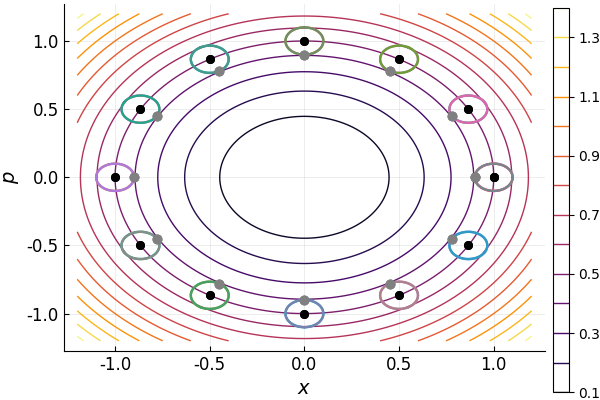
\includegraphics[width=0.8\linewidth]{oscillator_phsp}
 \caption{Espacio fase para el oscilador armónico representado por la ecuación \ref{eq:oscilador_ham}. En negro aparece la solución calculada con el método de Taylor para jets con $\xo = (1,0)^T$, tolerancia $\epsilon_{Taylor} = 10^{-20}$, orden de la expansión $M = 28$ y orden del jet $N=4$. Los jets fueron evaluados para la vecindad parametrizada por $\mathbf{\xi}(\tau) = 0.1\cdot \left( \cos(\tau), \sin(\tau) \right)^T$, $\tau \in [0,1]$, mientras que la solución en gris representa la variación $\xi = (-0.1,0)^T$.}
 \label{fig:oscilador_phsp}
\end{figure}

Así, tenemos que las soluciones analíticas son de la forma 
\begin{align}
 x(t) &= v_{0}\sin{(\omega t)} + x_{0}\cos{(\omega t)} \nonumber \\ 
 v(t) &= v_{0}\omega\cos{(\omega t)} - x_{0}\omega\sin{(\omega t)}. 
 \label{eq:oscilador_analytical}
\end{align}

La figura \ref{fig:oscilador_phsp} presenta al espacio fase del oscilador armónico, junto con una solución calculada con el transporte de jets. En ésta se observa cómo las soluciones evaluadas en una vecindad inicial parametrizada por un círculo están siempre en las líneas de las curvas de nivel del hamiltoniano. Se observa además en la figura la estructura de centros alrededor del único punto singular $(0,0)^T$.

Dada la condición inicial $\xo = (1,0)^T$ y tomando $m = 1 \ Kg$, $k = 1 \frac{Kg}{s^2}$, el oscilador tendrá una energía de $E_0 = H(\xo) = 1$ Joules. En la figura \ref{fig:oscillator_deltas} se pueden ver las variaciones $\delta E(t_n)$ de la energía en cada paso de integración así como la diferencia $\delta \mathbf{x}(t_n)$ de las soluciones de jet calculadas por el método de Taylor evaluadas en diferentes $\xi$s y las soluciones analíticas del oscilador armónico correspondientes al desplazamiento dado por dichas $\xi$s.

%FIGURA!
 \begin{figure}[h!]
\centering
\begin{subfigure}{0.49\textwidth}
	\centering
	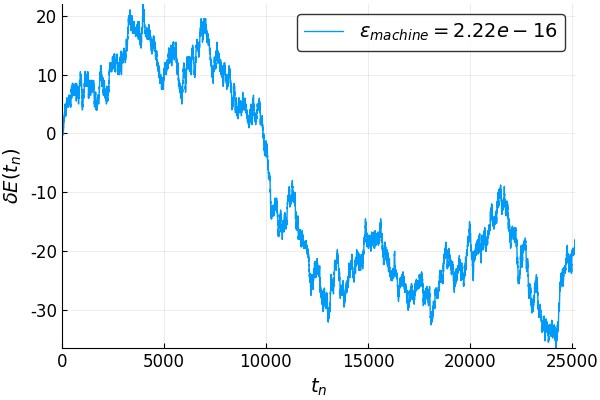
\includegraphics[width = \textwidth]{oscillator_dE}
	\caption{Variación $\delta E(t_n) = \frac{E(t_n)-E_0}{\epsilon_{machine}}$ de la energía respecto a la energía inicial $E_0 = 1$ Joule.\\ \\ }
	\label{fig:oscillator_dE}
\end{subfigure}
%
\begin{subfigure}{0.49\textwidth}
	\centering
	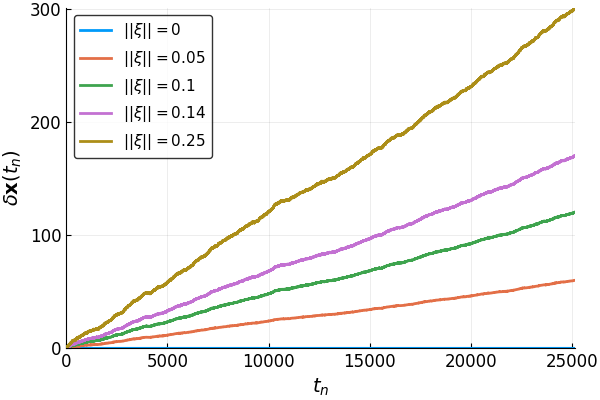
\includegraphics[width = \textwidth]{oscillator_dx}
	\caption{Variación $\delta \mathbf{x}(t) =  \frac{\norm{\mathbf{x}(t_n) - \mathbf{x_n}}_2}{\epsilon_{machine}}$ respecto a la solución analítica (\ref{eq:oscilador_analytical}) para distintos desplazamientos $\xi$ respecto de la condición inicial $\xo$.}
	\label{fig:oscillator_dx}
\end{subfigure}
\caption{Variaciones de energía y trayectoria para el oscilador armónico en cada uno de los pasos temporales de la solución con condición inicial $\xo = (1,0)^T$ y vecindad parametrizada por  $\mathbf{\xi}(\tau) = 0.1\cdot \left( \cos(\tau), \sin(\tau) \right)^T$, $\tau \in [0,1]$. Se utilizó tolerancia $\epsilon_{Taylor} = 10^{-20}$, orden de la expansión $M = 28$ y orden del jet $N=4$.}
\label{fig:oscillator_deltas}
\end{figure}

Es interesante notar que (\ref{eq:oscilador_ode}) es un sistema lineal de ecuaciones y, por tanto, basta con un jet de orden $1$ para obtener la mejor aproximación de las vecindades de $\xo$. De hecho, evaluar $\U_{\xo}$ en $f(\mathbf{x})$ de (\ref{eq:ode}) siempre regresa una cantidad lineal y por tanto, nunca aparecen términos de orden mayor en las variables del sistema de EDO.

\subsubsection{Péndulo simple}
\label{sec:pendulo}
Sea un sistema donde una masa $m$ está anclada al extremo de una varilla de longitud $l$ cuya masa es despreciable. Esta varilla está anclada, a su vez, a un punto inmovil. Así, $m$ se mueve bajo la acción de la gravedad $\mathbf{g}$ como se muestra en la figura \ref{fig:pendulo}, ignorando la resistencia del aire.

%FIGURA! 


La forma más natural de trabajar este problema es en coordenadas polares, en donde la masa $m$ se mueve con una velocidad $v = l\dot{\theta}$ con $l$ constante, es decir $r = l \neq r(t) \implies \dot{r} = \dot{p_r} = 0$. Esta constricción reduce en uno los grados de libertad del sistema, haciendo que éste dependa únicamente de $\theta$. 

Tenemos que 
\begin{align}
 K &= \frac{1}{2}m v^2 = \frac{1}{2} m l^2 \dot{\theta}^2 \nonumber \\
 U &= mgh(\theta) = mgl\left(1 - \cos{\theta} \right)
\end{align}
son la energía cinética y potencial, respectivamente. 

Así, contruimos el lagrangiano del sistema
\begin{equation*}
 \mathcal{L}(\theta,\dot{\theta}) = K - U = \frac{1}{2} m l^2 \dot{\theta}^2 - mgl\left(1 - \cos{\theta} \right).
\end{equation*}
Sabemos, por (\ref{eq:lagr-ham-rel}), que
\begin{equation*}
 \mathbf{p} = \frac{\partial \mathcal{L}}{\partial \mathbf{\dot{q}}} = ml^2\dot{\theta}
\end{equation*}

obteniendo la coordenada conjugada de momento y, así, plantear el hamiltoniano, o energía total del sistema, como
\begin{equation}
 H(p,\theta) = K + U = \frac{p_{\theta}^2}{2ml^2} + mgl\left(1 - \cos{\theta} \right).
\label{eq:pendulo-ham}
\end{equation}
 
Las EDO quedan entonces, por (\ref{eq:ham-rel}), como
\begin{align}
 \dot{\theta} &= \frac{p_{\theta}}{ml^2} \nonumber \\
 \dot{p_{\theta}} &= -mgl\sin{\theta} 
\label{eq:pendulo-ode}
\end{align}

en cuyo dominio $(\theta,p_{\theta}) \in [-\pi,\pi]\times[p_{min},p_{max}] \subset \mathbb{R}^2$ existen tres puntos singulares: $(-\pi,0),(\pi,0), (0,0)$; dos puntos de ``liberación'' y otro de ``relajación'', respectivamente. En la figura \ref{fig:pendulum_pshp} se puede ver una representación del espacio fase donde se exhibe el comportamiento de dichos puntos.

%FIGURA!
\begin{figure}[h!]
 \centering
 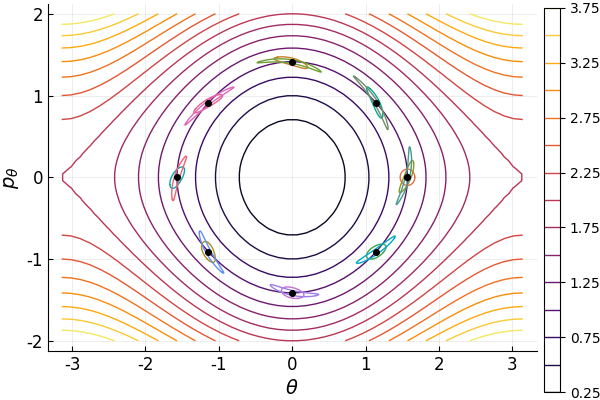
\includegraphics[width=0.8\linewidth]{pendulum_phsp}
 \caption{Espacio fase para el péndulo simple representado por la ecuación \ref{eq:pendulo-ham}. En negro salen puntos de la trayectoria calculada con el método de Taylor para Jets con $\xo = (\frac{\pi}{2},0)^T$, tolerancia $\epsilon_{Taylor} = 10^{-20}$, orden de la expansión $M = 28$ y sus vecindades (jets) evaluadas para $\mathbf{\xi}(\tau) = 0.1\cdot \left( \cos(\tau), \sin(\tau) \right)^T$, $\tau \in [0,1]$.}
\label{fig:pendulum_pshp}
\end{figure}

Si viajamos a un planeta en donde $g = 1 \ \frac{m}{s^2}$ \footnote{A veces, para la física, es más fácil viajar a un planeta donde exista la atracción gravitacional que más nos gusta que hacer a un péndulo girar en la Tierra; qué comodo.} y tomamos una varilla de longitud $l=1$ m y una masa $m=1$ kg,  entonces, para las condiciones iniciales $p_{\theta}(0) = 0 \ N \cdot m$ y $\theta(0) = \pi/2$, la energía total es 
\begin{equation*}
E_0 = H(p_{\theta}(0),\theta (0) ) = 1 \text{ J.}
\end{equation*}

Para dichas condiciones, se puede integrar el transporte de jets y además, evaluarlo para condiciones cercanas y ver cómo se comportan éstas soluciones en el espacio fase, que deben, en teoría, moverse por las curvas de (\ref{eq:pendulo-ham}). Se puede observar de la figura \ref{fig:pendulum_jt} cómo para jets de orden 4, las soluciones se quedan sobre las curvas de nivel del hamiltoniano.

%FIGURA!
\begin{figure}[h!]
\centering
\begin{subfigure}{0.49\textwidth}
	\centering
	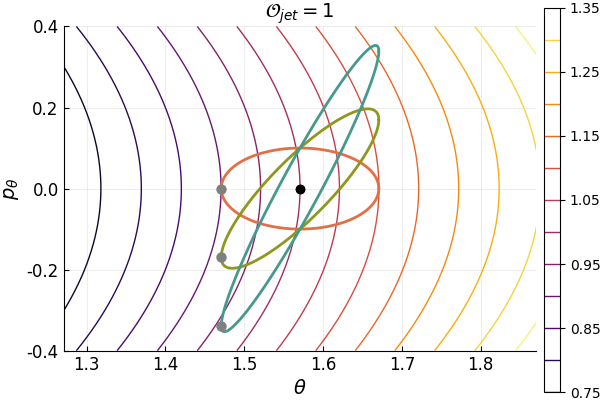
\includegraphics[width = \textwidth]{pendulum_jt_O1}
	\caption{Jet de orden $1$ después de dos periodos desde $\xo$.}
	\label{fig:pendulum_jt_O1}
\end{subfigure}
%
\begin{subfigure}{0.49\textwidth}
	\centering
	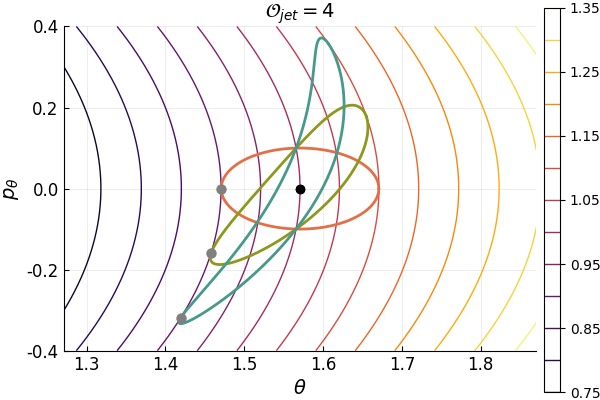
\includegraphics[width = \textwidth]{pendulum_jt_O4}
	\caption{Jet de orden $4$ después de dos periodos desde $\xo$.}
	\label{fig:pendulum_jt_O4}
\end{subfigure}
\caption{Jets de distinto orden para $\U_{\xo}$ parametrizada en un círculo de radio 0.1 $\mathbf{\xi}(\tau) = 0.1\left( \cos(\tau),\sin(\tau) \right)^T$ alrededor de $\xo = (\frac{\pi}{2},0)^T$ en el péndulo simple. Se utilizó tolerancia $\epsilon_{Taylor} = 10^{-20}$ y orden de la expansión $M = 28$.}
\label{fig:pendulum_jt}
\end{figure}

Respecto a las variaciones de energía en el sistema, se ve en la figura \ref{fig:pendulum_dE} cómo $\delta E(t)$ varía alrededor de cero como un movimiento browniano. Éste último se relaciona con los errores de redondeo de puntos flotantes de la máquina y no con el método de Taylor en sí, a diferencia del método de Euler, como se observa en la figura \ref{fig:center_anal_comparison}, donde el error crece de manera lineal. La máxima variación respecto a la energía inicial es de $2.28\times10^{-14}$, lo cual corresponde a $103 \epsilon_{machine}$ (sin redondear).

%FIGURA! 
\begin{figure}[h!]
 \centering
 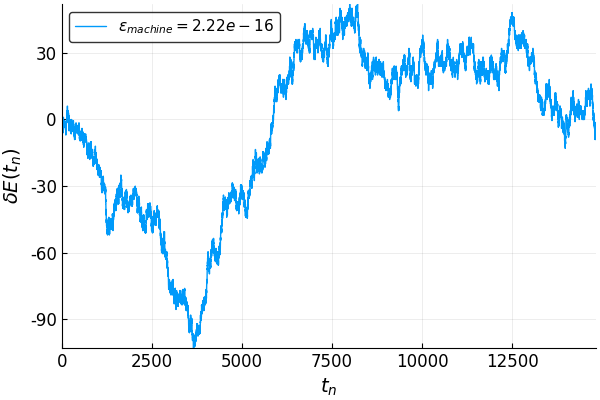
\includegraphics[width=0.8\linewidth]{pendulum_dE}
 \caption{Diferencia $\delta E(t_n) := \frac{E(t_n) - E_0}{\epsilon_{machine}}$ de la energía del péndulo simple con condición inicial $\xo = (\frac{\pi}{2},0)$, tolerancia $\epsilon_{Taylor} = 10^{-20}$ y orden de la expansión $M = 28$.}
 \label{fig:pendulum_dE}
\end{figure}

\subsubsection{Hamiltoniano Artificial}
\label{sec:artificial_ham}

Inventemos un hamiltoniano que no necesariamente represente un sistema físico. Éste último ejemplo servirá como motivación de la sección siguiente, ya que estaremos analizando las soluciones cerca de una curva límite y se podrá extender un poco la discusión sobre los jets y la necesidad de contruir algunos indicadores dinámicos relevantes. 

Sea 
\begin{equation}
 H(q,p) = qp^2 - \frac{1}{2}q^2
 \label{eq:artificial_ham}
\end{equation}

el hamiltoniano del sistema cuyas curvas de nivel representan las soluciones para la EDO
\begin{align}
 \dot{q} &= 2qp \nonumber \\
 \dot{p} &= -p^2 + q.
 \label{eq:artificial_ode}
\end{align}


Notemos que el sistema anterior tiene un único punto singular $(0,0)^T$ que corresponde a una energía de $H(0,0) = 0$. Con esto, podemos obtener la condición para que las soluciones estén sobre dicho curva límite o separatriz que divide diferentes regiones del espacio. Vemos que si
\begin{equation*}
 H(q,p) = qp^2 - \frac{1}{2}q^2 = 0 \implies p = \pm \sqrt{\frac{q}{2}} 
\end{equation*}

entonces las condiciones iniciales tipo $\xo = \left( q, -\sqrt{\frac{q}{2}} \right)$ vivirán sobre la separatriz. 

%FIGURA!
\begin{figure}[h!]
 \centering
 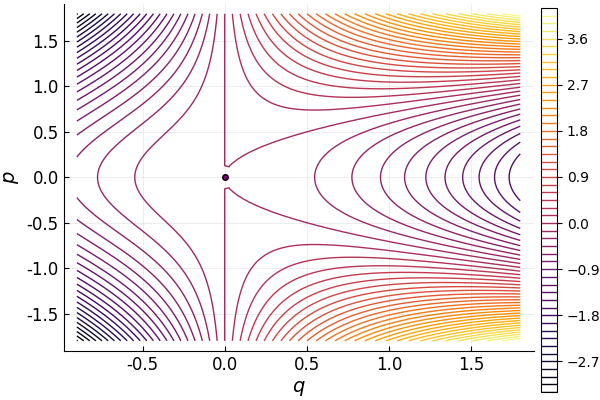
\includegraphics[width= 0.8\linewidth]{artificial_phsp}
 \caption{Espacio fase de \ref{eq:artificial_ode}.}
 \label{fig:artificial_phsp}
\end{figure}

Se muestra en la figura \ref{fig:artificial_phsp} el espacio fase dado por el hamiltoniano del sistema. Notemos que dicha separatriz se puede observar como una especie de parábola horizontal positiva con centro en el punto singular.

%FIGURA!
\begin{figure}[h!]
 \centering
 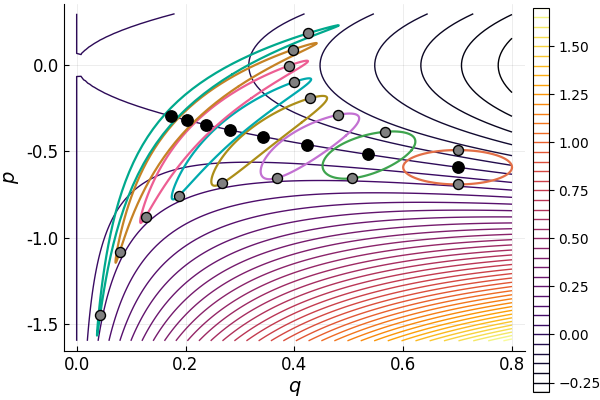
\includegraphics[width= 0.8\linewidth]{artificial_jt_O16}
 \caption{Solución para (\ref{eq:artificial_ode}), con condición inicial sobre la separatriz, donde $q_0 = 0.7$. Aquí, los jets son de orden $M=16$, en $8$ pasos de integración desde $t_0 = 0$ hasta $t_{max} = 1.7$, con tolerancia $\epsilon_{Taylor} = 10^-{20}$ y orden de la expansión $N=28$. En gris están las soluciones a $\xo + \xi$ sin utilizar TJ.}
 \label{fig:artificial_jt}
\end{figure}

Si tomamos $q_0 = 0.7$ con la condición anterior, y hacemos un transporte de jets alrededor de dicha condición inicial podríamos ver, en teoría, las trayectorias que toman las soluciones cercanas a la curva límite en cada lado de la frontera que ésta impone. En la figura \ref{fig:artificial_jt} se observa la deformación de estos jets conforme pasa el tiempo y, aunque la evolución temporal es un intervalo relativamente corto, es evidente la tendencia que tienen las soluciones cercanas a diverger.

En este problema se vuelve importante muy rápidamente la precisión con la que los jets nos dan soluciones cercanas ya que la deformación de la vecindad inicial $\U_{\xo}$ es muy grande. Por esto, se muestra en la tabla \ref{table:djet_artificial} la diferencia entre evaluar el jet en $\xi = (0,-0.1)^T$ y hacer el método de Taylor convencional partiendo de ese punto. De hecho, se observan en la figura \ref{fig:artificial_jO2_jO16} la evaluación de jets de distinto orden para la misma vecindad inicial alrededor de $\xo$.

%TABLA!
\begin{table}[h!]
\centering
\begin{tabular}{c|ccccc}
\toprule
               & \textbf{$ M = 1 $} & \textbf{$M = 2 $} & \textbf{$ M = 4$} & \textbf{$ M = 8 $} & \textbf{$ M = 16 $} \\ \cmidrule(l){1-6} 
\textbf{$t_0$} & -Inf                       & -Inf                       & -Inf                       & -Inf                       & -Inf                          \\
\textbf{$t_1$} & -2.42                      & -3.97                      & -7.07                      & -13.28                     & -15.95                        \\
\textbf{$t_2$} & -1.92                      & -3.1                       & -5.47                      & -10.22                     & -15.95                        \\
\textbf{$t_3$} & -1.54                      & -2.48                      & -4.37                      & -8.15                      & -15.91                        \\
\textbf{$t_4$} & -1.21                      & -1.96                      & -3.47                      & -6.49                      & -12.53                        \\
\textbf{$t_5$} & -0.91                      & -1.49                      & -2.68                      & -5.05                      & -9.79                         \\
\textbf{$t_6$} & -0.61                      & -1.05                      & -1.95                      & -3.74                      & -7.34                         \\
\textbf{$t_7$} & -0.29                      & -0.6                       & -1.24                      & -2.52                      & -5.08                         \\ \bottomrule 
\end{tabular}
\caption{Diferencia logarítmica de $\delta \mathbf{x} = \norm{ \phi(t_i,t_0,\xo + (0,-0,1)^T) - P_{i,\xo}((0,-0.1)^T) }$ para polinomios $P_{i,\xo}(\xi)$ de distinto orden $M$ en $\xi$.}
\label{table:djet_artificial}
\end{table}

%FIGURA!
\begin{figure}[h!]
 \centering
 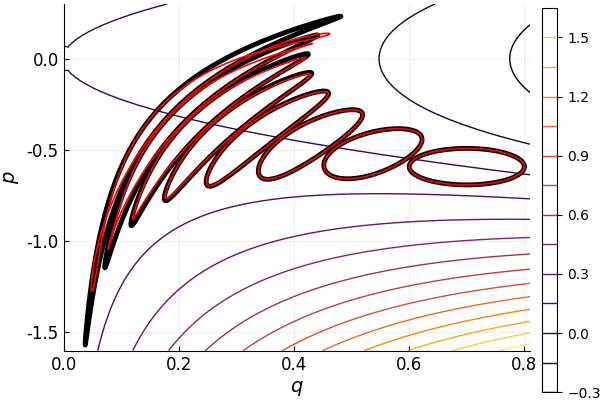
\includegraphics[width= 0.7\linewidth]{artificial_jO2_jO16}
 \caption{Diferencia gráfica entre un jet de orden $M=2$ contra uno de orden $M=16$ para las mismas condiciones.}
 \label{fig:artificial_jO2_jO16}
\end{figure}

Recordemos que como \ref{eq:artificial_ode} es un sistema de EDO hamiltoniano entonces deberá conservar la energía. En la figura \ref{fig:artificial_dE} se observa la variación de la energía para cada paso temporal con el jet evaluado en $\xi = (0,\pm 0.1)^T$, así como en $\xo$, i.e., para el método de Taylor sin jets. Notemos cómo al principio (figura \ref{fig:}) la energía sí se conserva, i.e, las evaluaciones del TJ se mantienen sobre las superficies de nivel del hamiltoniano, sin embargo, cuando la vecindad se empieza a deformar más, la energía empieza a variar más respecto a la de su condición inicial. Notemos que aunque esta variación es de $\approx 10^8 \epsilon_{machine}$, el error en la energía es en la octava cifra significativa, dado que $\epsilon_{machine} = 2.22\times 10^{-16}$.

%FIGURA!
\begin{figure}[h!]
 \centering
 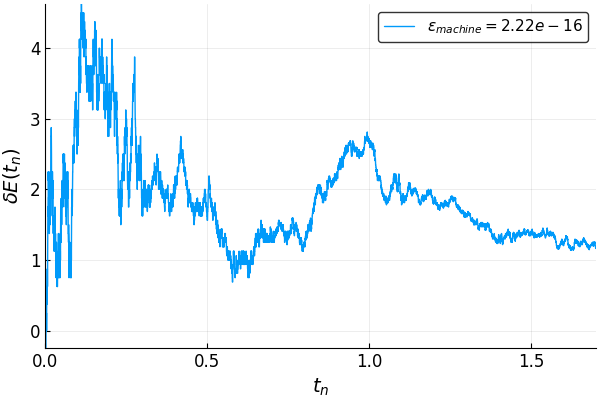
\includegraphics[width=0.7\linewidth]{artificial_dE}
 \caption{Diferencia en energía $\delta E(t_n) = \frac{1}{\epsilon_{machine}} \left( H(\mathbf{x}(t_n)) - H(\xo) \right)$ para el sistema \ref{eq:artificial_ode} sin transporte de jets, con tolerancia $\epsilon_{Taylor} = 10^{-20}$, orden de expansión $N = 28$ y $8000$ pasos temporales de $t_0 = 0$ a $t_{max} = 1.7$.}
 \label{fig:artificial_dE}
\end{figure}

%FIGURA!
\begin{figure}[h!]
\centering
\begin{subfigure}{0.49\textwidth}
	\centering
	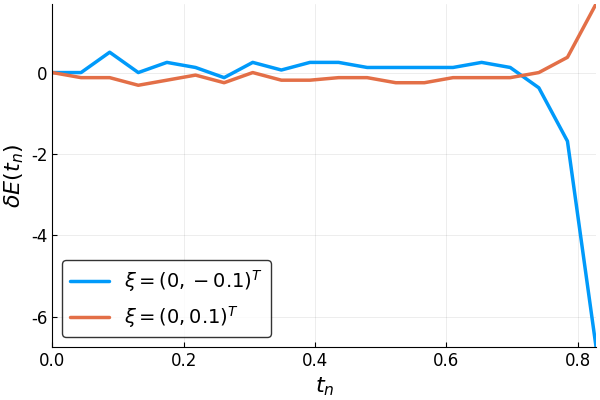
\includegraphics[width = \textwidth]{artificial_dEjets_half}
	\caption{Diferencias de energía $\delta E$ respecto a la energía inicial en la primera mitad de la integración.}
	\label{fig:artificial_dEjets_half}
\end{subfigure}
%
\begin{subfigure}{0.49\textwidth}
	\centering
	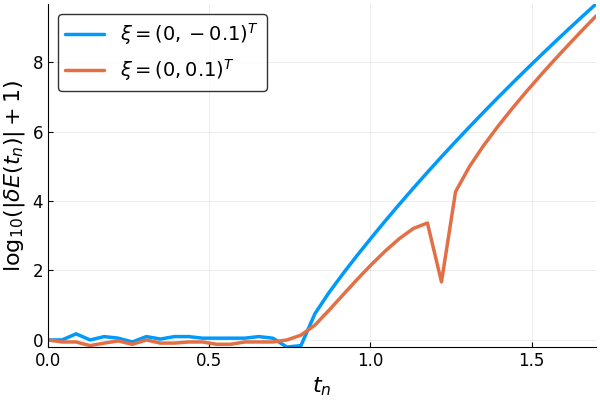
\includegraphics[width = \textwidth]{artificial_dEjets_all}
	\caption{Logaritmo de las diferencias de energía $\delta E$ respecto a la energía inicial en toda la integración.}
	\label{fig:artificial_dEjets_all}
\end{subfigure}
\caption{Diferencia en energía $\delta E(t_n) = \frac{1}{\epsilon_{machine}} \left( H(\mathbf{x}(t_n)) - H(\xo) \right)$ para el sistema (\ref{eq:artificial_ode}) con jets de orden $M=16$ evaluados en $\xi$. Se utilizó tolerancia $\epsilon_{Taylor} = 10^{-20}$, orden de expansión $N = 28$ y $40$ pasos temporales de $t_0 = 0$ a $t_{max} = 1.7$.}
\label{fig:pendulum_jt}
\end{figure}


Todos los ejemplos construidos en la última sección han sido evaluados en una vecindad con un radio de $r = 0.1$ alrededor de $\xo$. Sin embargo, nada asegura que ésta sea una buena elección para dicha vecindad. Estudiar cuál es el tamaño máximo que una vecindad puede tomar para que los jets arrojen soluciones precisas se vuelve una pregunta natural al ver las gráficas y tablas de éstos ejemplos. Por otro lado, hemos visto en éste último ejemplo cómo una vecindad inicial puede deformarse bastante rápido cerca de una curva límite cuando en el oscilador armónico, en cambio, no se deforma nada. Establecer una métrica de deformación se vuelve, también, una forma de análisis del estudio de vecindades de alguna condición $\xo$ dada para algún sistema de ecuaciones diferenciales a trabajar. En el caso del péndulo simple, se observa cómo después de cada periodo de oscilación, el jet se deforma de manera tal que las soluciones cercanas no cruzan la condición inicial al mismo tiempo que $\xo$; esto se puede estudiar si pintamos una sección transversal a las soluciones del péndulo que pase por $xo$ y observamos en qué tiempo cruzan las vecindades ésta sección. El uso de jets motiva a hacer varios indicadores sobre la dinámica de las ecuaciones son obtener explícitamente la solución. Es importante notar que no siempre se tendrá un hamiltoniano explicito para comparar las soluciones con sus curvas de nivel, así que estos indicadores servirán para darnos información sobre el espacio fase sin conocerlo del todo. 

Los siguientes indicadores están motivados fuertemente en lo discutido en \cite{Perez2015}, \cite{Perez2015}, \cite{Haro2009}.